\begin{abstract}
GlareShell (Feng et al., Computer Networks 2024) detects PHP webshells by turning each script into an
interprocedural control-flow graph (ICFG) of statements, embedding the statements, adding a risk level per statement
and classifying the graph with a GNN; it reports F1 = 0.9887. Neither code nor data were released. We re-implement
the pipeline on the same static-analysis tool (with four fixes needed for modern PHP), rebuild the corpus from the
paper's sources with provenance and near-duplicate clusters, and run every experiment with five seeds and paired
significance tests. On the paper's protocol we reproduce the headline result (F1 0.98) but not the finer claims: GAT is
not better than GCN or GIN, and normalisation and risk weights do not significantly help. Beyond the paper, 77\% of
test webshells in a random split have a near-duplicate in training, a TF-IDF + logistic-regression baseline beats
every GNN, and on four unseen benign projects the false-positive rate quadruples; at a 0.1\% alarm budget GAT finds
only 6\% of unseen webshells (text baseline: 64\%), and 10 of 12 hand-written legitimate scripts are flagged. Adding
five small benign applications to training cuts the GAT false-positive rate from 2.5\% to 0.9\% without a significant
loss of recall. High scores on this benchmark mostly measure the difference between framework code and webshell
collections, not malicious behaviour.
\end{abstract}

\begin{IEEEkeywords}
webshell detection, graph neural networks, PHP, reproducibility, data leakage, dataset quality
\end{IEEEkeywords}

\section{Introduction}\label{sec:intro}
A \emph{webshell} is a server-side script planted in the web root after an initial compromise (unrestricted upload,
LFI/RFI, SQL injection, stolen credentials) that gives a remote party control of the server through ordinary HTTP
requests (MITRE ATT\&CK T1505.003~\cite{mitre_t1505003}). Families range from one-line backdoors
(\verb|<?php @eval($_POST['x']);?>|) and command shells over large management kits (c99, r57, WSO, b374k) to
obfuscated loaders (\verb|eval(gzinflate(base64_decode('...')))|, \verb|$f='as'.'sert'; $f($_REQUEST[k]);|) and
plain uploaders. GlareShell~\paperref{} targets the Industrial-Internet setting, where the web server is the management
plane of control systems, and detects webshells \emph{statically}: a file-system monitor inspects every new or
modified \texttt{.php} file before it runs. The defender sees only the source file; a false positive blocks a
legitimate deployment, a false negative leaves a backdoor.
\begin{figure*}[!t]
\centering
\resizebox{\linewidth}{!}{%
\begin{tikzpicture}[
  box/.style={draw,rounded corners=2pt,align=center,font=\footnotesize,inner sep=3pt,minimum height=7mm},
  att/.style={box,fill=red!8}, obs/.style={box,fill=blue!8}, det/.style={box,fill=green!10}, conf/.style={box,fill=orange!12},
  ->,>=Stealth]
\node[att] (vuln) {Initial access\\upload / LFI / SQLi /\\stolen credentials};
\node[att,right=8mm of vuln] (drop) {Webshell file\\written to web root};
\node[att,right=8mm of drop] (req) {Attacker HTTP\\request (\texttt{\$\_POST}, cookie,\\header)};
\node[att,right=8mm of req] (act) {Command / code exec,\\file ops, DB access,\\pivot to OT network};
\draw (vuln)--(drop); \draw (drop)--(req); \draw (req)--(act);
\node[obs,below=10mm of drop] (fs) {\textbf{Observation surface}\\new/modified \texttt{.php} file\\(file-system monitor)};
\draw[dashed] (drop)--(fs);
\node[det,right=8mm of fs] (icfg) {Static view: ICFG of\\PHP statements\\(normalised + risk level)};
\node[det,right=8mm of icfg] (gnn) {GNN classifier\\$\rightarrow$ allow / block};
\draw (fs)--(icfg); \draw (icfg)--(gnn);
\node[box,below=8mm of fs,fill=gray!8] (fam) {Families: one-liner $\cdot$ command shell $\cdot$ kit $\cdot$\\obfuscated loader $\cdot$ uploader};
\node[conf,below=8mm of icfg,xshift=14mm] (conf) {Confusable: benign code with exec/callbacks;\\webshells with only dynamic calls or hidden payloads};
\draw[dotted] (fam)--(fs); \draw[dotted] (conf)--(icfg);
\node[box,left=8mm of fs,fill=gray!8] (evade) {Evasion: string building,\\encoding, callbacks,\\short tags, padding};
\draw[dotted] (evade)--(fs);
\end{tikzpicture}}
\caption{Concept map: attack chain (red), what the detector observes (blue), the detector (green) and
the sources of confusion we analyse (orange).}
\label{fig:concept}
\end{figure*}
\begin{table*}[!t]
\centering\small
\caption{Feature view of GlareShell (per node of the ICFG unless stated).}
\label{tab:features}
\begin{tabularx}{\linewidth}{@{}lXl@{}}
\toprule
Feature & Content & Malicious signal it can carry \\ \midrule
Statement text & One PHP statement / branch condition, pretty-printed & API used, request input, payload strings \\
Normalisation & local variables $\to$ \texttt{\$local}, user functions/methods $\to$ \texttt{user\_define}, numbers $\to$ \texttt{im} & removes names/passwords, keeps built-ins and strings \\
Embedding & 100-d vector of the normalised statement (W2V / FastText / GloVe / D2V) & co-occurrence of risky statements \\
Risk level & one-hot: 2 = \emph{critical} (\texttt{system, exec, shell\_exec, passthru, popen, proc\_open, pcntl\_exec}, backticks); 1 = \emph{obfuscated} (\texttt{eval, assert, preg\_replace, create\_function, call\_user\_func*}, array/sort callbacks, \dots); 0 = normal & explicit dangerous capability \\
Edges & intra-procedural control flow + call/return edges between functions (ICFG) & how input reaches the sink \\
Graph & mean of final node states (Eq.~6 of~\paperref{}) & whole-file behaviour \\
\bottomrule
\end{tabularx}
\end{table*}

\paragraph{Threat model} \emph{Attacker}: remote, already able to write a file into the web root, may obfuscate but
does not adapt to the specific model. \emph{Defender}: sees only the PHP source at creation/modification time -- no
execution traces, HTTP logs or file-system context -- and must decide per file before it runs. \emph{Out of scope}:
memory-resident and non-PHP shells, adaptive attacks, legitimately deployed admin tools. \Cref{fig:concept} relates the
attack chain, the observation surface and the sources of confusion we analyse; \Cref{tab:features} lists exactly what
GlareShell observes per file. The feature view predicts where it should fail: benign frameworks are full of
\emph{obfuscated}-level calls (\texttt{call\_user\_func\_array} for dispatch, \texttt{usort} with closures); webshells that
call dangerous functions only dynamically (\verb|$f(...)|) or hide the payload in an encoded string get no risk signal.

We reproduce GlareShell from its description and ask whether its performance measures what it claims to measure:
\begin{description}
  \item[RQ1] Can the reported performance (Tables 2 and 4 of~\paperref{}) be reproduced from the paper's sources?
  \item[RQ2] Do normalisation, risk weights, the embedding and the GNN contribute as claimed?
  \item[RQ3] How much of the score is explained by near-duplicate leakage and by the source confound?
  \item[RQ4] How does the detector behave on benign projects and webshells outside the training sources?
\end{description}
Contributions: (1) a working re-implementation including four extractor fixes; (2) a rebuilt, documented corpus
(GlareShell-R) with hashes, provenance, near-duplicate clusters and leakage-controlled splits; (3) a 5-seed replication
with paired tests; (4) leakage, baseline, alarm-budget and out-of-source analyses; (5) an improvement experiment.
An extended version with all tables (corpus funnel, extraction statistics, sweeps, ablation, per-project FPR, error
taxonomy, hyper-parameters) is in the repository (\texttt{report/extended.pdf}).

\section{GlareShell and our re-implementation}\label{sec:method}
\paragraph{Original pipeline}
(1) \emph{ICFG extractor}: LChecker~\cite{li2021lchecker} (on PHP-Parser~\cite{phpparser}) builds one CFG per function;
the paper's Algorithm~1 links them through call and return edges into an ICFG whose nodes are PHP statements, and
``meaningless'' statements are pruned. (2) \emph{Node attributes}: statements are normalised (local variables $\to$
\texttt{local}, user functions $\to$ \texttt{user-define}, numbers $\to$ \texttt{im}) and embedded with one of six
models (Word2Vec CBOW/Skip-gram~\cite{mikolov2013word2vec}, FastText~\cite{bojanowski2017fasttext},
GloVe~\cite{pennington2014glove}, Doc2Vec DM/DBOW~\cite{le2014doc2vec}); a one-hot risk level is appended:
\emph{critical} (\texttt{system}, \texttt{exec}, \texttt{shell\_exec}, \texttt{passthru}, \texttt{popen}, backticks, \dots),
\emph{obfuscated} (\texttt{eval}, \texttt{assert}, \texttt{create\_function}, \texttt{call\_user\_func*}, callbacks,
\dots) or normal. (3) \emph{Classifier}: GCN~\cite{kipf2017gcn}, GAT~\cite{velickovic2018gat} or GIN~\cite{xu2019gin},
mean pooling and an MLP. Reported: FastText best embedding (F1 0.945), GAT best GNN (F1 0.989) on 3,104 webshells and
10,375 benign files split randomly 8:1:1.

\begin{figure*}[!t]
\centering
\resizebox{\linewidth}{!}{%
\begin{tikzpicture}[box/.style={draw,rounded corners=2pt,align=center,font=\footnotesize,inner sep=3pt,minimum height=9mm,fill=gray!6},->,>=Stealth]
\node[box] (a) {\texttt{fetch\_sources.sh}\\15 repos, pinned};
\node[box,right=5mm of a] (b) {\texttt{build\_manifest.py}\\hashes, provenance,\\2-level dedup};
\node[box,right=5mm of b] (c) {\texttt{extract\_icfg.php}\\LChecker CFG + Alg.~1\\prune, normalise, risk};
\node[box,right=5mm of c] (d) {\texttt{splits.py}\\MinHash near-dup\\protocols $\times$ 5 seeds};
\node[box,right=5mm of d] (e) {\texttt{embeddings.py}\\6 methods,\\train split only};
\node[box,right=5mm of e] (f) {\texttt{train\_gnn.py}\\GCN/GIN/GAT\\+ baselines};
\node[box,right=5mm of f] (g) {\texttt{analyze.py}\\tables, CIs,\\paired tests};
\draw (a)--(b); \draw (b)--(c); \draw (c)--(d); \draw (d)--(e); \draw (e)--(f); \draw (f)--(g);
\end{tikzpicture}}
\caption{Reproduction pipeline (one script per box in \texttt{src/}). Samples are only parsed; nothing is executed.}
\label{fig:pipeline}
\end{figure*}

\paragraph{Our implementation (\Cref{fig:pipeline})}
LChecker's own analysis is a taint checker that outputs no graphs, but its CFG builder is reusable; we call it unchanged
and implement Algorithm~1, pruning, AST-level normalisation and risk levels on top (\texttt{src/php/extract\_icfg.php}).
Four problems not mentioned by the paper had to be fixed: (i) LChecker silently skips \texttt{namespace},
\texttt{try/catch} and \texttt{declare} blocks, so vanilla LChecker yields \emph{empty graphs for most modern framework
files} -- a perfect label leak; we flatten these blocks. (ii) \texttt{for} conditions crash the pretty-printer
(854 files). (iii) PHP~8 disables short open tags, so 208 webshells (and no benign file) parse as HTML; we parse with
\texttt{short\_open\_tag=On}. (iv) Two files segfault PHP and are kept as empty graphs. ICFGs are capped at 2,000
statements (15\% of webshells, 0.4\% of benign files). Embeddings use Gensim defaults (dimension 100, window 5) and are
\textbf{trained only on the training files of each split and seed}, so no test statement leaks into them. GNNs use
PyTorch Geometric with the paper's hyper-parameters (Table~2 setting: 2-layer GCN, hidden 10; Table~3 optimum:
3 layers, batch 256, 120 epochs); model selection uses validation F1.

\section{Dataset: GlareShell-R}\label{sec:dataset}
\paragraph{Sources}
We cloned every repository of the paper's Table~1 at pinned revisions. \texttt{ysrc/webshell-sample} has been deleted;
its files survive only inside the Cyc1e183 aggregate~\cite{cyc1e183} (2,917 webshells from 17 collections, named by MD5,
no origin), which dominates the webshell side. Benign files come from WordPress, Drupal, Laravel, PHPMailer and doorGets.
After exact-hash deduplication we obtain \textbf{3,097 webshells} (paper: 3,104, so the paper used exact
deduplication) and subsample 10,375 benign files as in the paper. For generalisation we add four \emph{held-out} benign
projects (Laravel framework, phpMyAdmin, Joomla, Matomo) and two held-out webshell collections. Every file has a SHA-256,
source, revision and path in the manifest; a data card, schema and label guide are in \texttt{docs/}.

\paragraph{Extraction is label-dependent}
\Cref{tab:extraction} shows that webshells are older, less well-formed and much larger: 4.5\% contain syntax errors,
15.4\% exceed the 2,000-statement cap (benign: 0.4\%), and their statement counts span four orders of magnitude
(\Cref{fig:stmtdist}). These are signals a classifier can exploit without understanding behaviour.
\begin{table*}[!t]
\centering\footnotesize
\caption{ICFG extraction outcome (after the four extractor fixes of \Cref{sec:method}).}
\label{tab:extraction}
\begin{tabular}{@{}llrrrrrrrr@{}}
\toprule
Label & Subset & Files & Crash & Parse err. & Empty ICFG & Truncated & Median nodes & P90 nodes & ms/file \\ \midrule
benign & heldout & 9101 & 0 & 1 & 123 & 7 & 18 & 103 & 6.9 \\
benign & paper & 12930 & 0 & 1 & 590 & 49 & 14 & 99 & 7.9 \\
webshell & heldout & 46 & 0 & 7 & 3 & 4 & 25 & 755 & 26.6 \\
webshell & paper & 3097 & 4 & 139 & 53 & 477 & 11 & 875 & 36.6 \\
\bottomrule
\end{tabular}

\end{table*}

\begin{figure*}[!t]
\centering
\subfloat[Statements per webshell ICFG (cf.\ paper Fig.~5).\label{fig:stmtdist}]{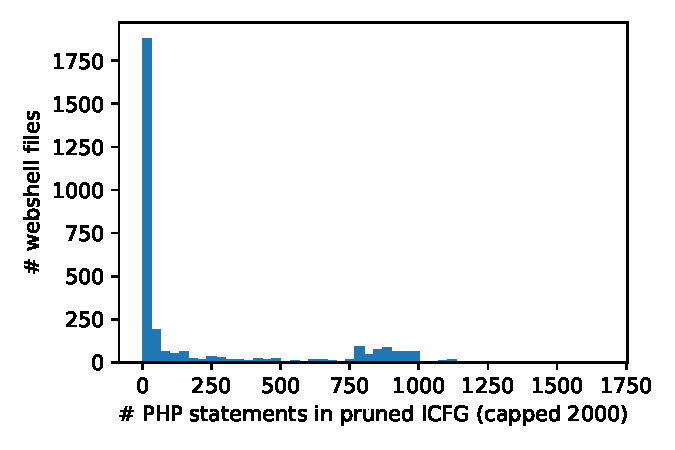
\includegraphics[width=0.42\linewidth]{figures/stmt_dist.pdf}}\hfil
\subfloat[Near-duplicate cluster sizes, paper webshells.\label{fig:clusters}]{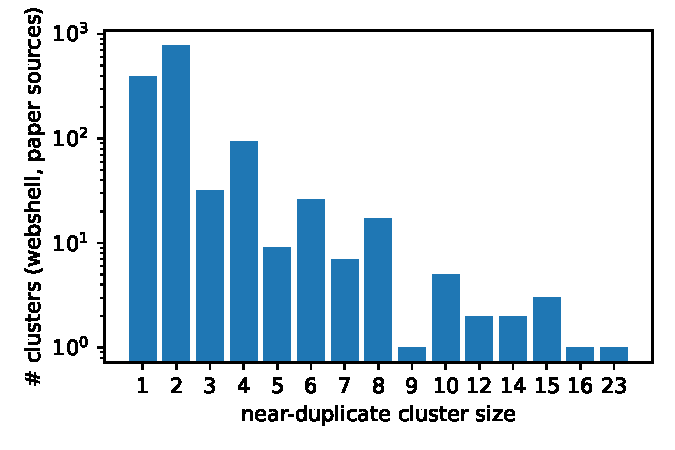
\includegraphics[width=0.42\linewidth]{figures/cluster_sizes.pdf}}
\caption{Corpus structure.}
\end{figure*}

\paragraph{Near-duplicates}
1,265 of the 2,917 Cyc1e183 files (43\%) are identical once whitespace is removed. Clustering files by the set of their
normalised statements (MinHash-LSH~\cite{broder1997minhash}, Jaccard $\ge 0.8$) collapses the 3,097 webshells into
1,368 clusters (largest: 55 members, \Cref{fig:clusters}) (benign: 12,930 $\to$ 11,828). In the paper's random split \textbf{77.0\% $\pm$ 4.4\% of test webshells
have a near-duplicate in training} (benign: 9\%), so its test set mostly measures recognition of known
families~\cite{allamanis2019duplication,arp2022dos}.

\paragraph{Evaluation protocols} (5 seeds each)
\begin{description}
  \item[\pr] the paper's protocol: exact dedup, stratified random 8:1:1.
  \item[\cg] leakage-controlled: whitespace dedup; whole near-duplicate clusters go to train, validation or test.
  \item[\xs] generalisation: trained as \cg; tested on 9,091 files of the four unseen benign projects and the 18
        webshells that share no cluster with the paper corpus -- primarily a \emph{false-positive} stress test.
  \item[\texttt{loo}] leave-one-collection-out: all webshells first published in one collection (tennc 222, bartblaze 99,
        xl7dev 77) and every cluster they touch are held out.
\end{description}
A temporal split is impossible: 93\% of webshells share one commit date (the Cyc1e183 upload, 2020-11-13).

\section{Experimental setup}\label{sec:setup}
Hardware: RTX~3050 6\,GB, 7.6\,GB RAM; PyTorch~2.4.1, PyG~2.6.1, Gensim~4.3.3, PHP~8.3. Positive class = webshell; we
report the paper's precision, recall, TNR and F1 plus FPR, the quantity that decides deployability. Every configuration
runs with 5 seeds (mean $\pm$ 95\% Student-$t$ half-width); key comparisons use a paired $t$-test on per-seed F1 and an
exact McNemar test on per-file decisions. \textbf{Baselines} on the same splits: TF-IDF of lexical PHP tokens (1--2-grams)
with logistic regression or XGBoost; rules built from GlareShell's own risk lists; and \emph{graph statistics} +
XGBoost -- twelve numbers per ICFG (size, density, number of risky statements, parse error, \dots) with no code
semantics, a probe for corpus artefacts.

\section{Results}\label{sec:results}
\subsection{Reproducing the paper (RQ1, RQ2)}\label{sec:repro}
\Cref{tab:repro} compares our F1 with the paper. The headline is reproduced: all three GNNs reach F1 $\approx$ 0.98
(paper 0.968--0.989), and FastText is the best embedding by a significant margin (paired $p=0.007$, McNemar
significant in 5/5 seeds). The finer claims are not: (i) the five other embeddings lie within 0.036 F1 with
overlapping intervals and a different order; (ii) GAT is \emph{not} the best GNN -- GAT vs.\ GCN $p=0.79$, vs.\ GIN
$p=0.48$; (iii) F1 is flat over embedding dimensions 20--120 (0.978--0.981) and windows 2--7, with no rise-then-fall (\Cref{fig:sweeps});
(iv) normalisation and risk weights do not significantly help ($p=0.10$ on \pr), and on \cg{} raw statements without
either are nominally best ($p=0.07$, \Cref{fig:ablation}); normalisation removes names and literals that help to recognise near-duplicates in a random split. \Cref{tab:signif} lists all paired tests.

\begin{table}[!t]\centering\footnotesize
\caption{F1 on \pr{} (5 seeds) vs.\ the paper. Top: Table 2 (embeddings, 2-layer GCN); bottom: Table 4 (FastText).}\label{tab:repro}
\begin{tabular}{@{}lrrr@{}}\toprule
Setting & Ours & Paper & $\Delta$ \\ \midrule
GloVe & 0.928 $\pm$ 0.013 & 0.914 & +0.015 \\
Word2Vec CBOW & 0.899 $\pm$ 0.025 & 0.937 & $-$0.038 \\
Word2Vec Skip-gram & 0.915 $\pm$ 0.012 & 0.936 & $-$0.021 \\
Doc2Vec DM & 0.912 $\pm$ 0.020 & 0.931 & $-$0.019 \\
Doc2Vec DBOW & 0.935 $\pm$ 0.018 & 0.929 & +0.006 \\
\textbf{FastText} & \textbf{0.977 $\pm$ 0.009} & \textbf{0.945} & +0.032 \\ \midrule
GCN & 0.981 $\pm$ 0.008 & 0.968 & +0.013 \\
GIN & 0.983 $\pm$ 0.002 & 0.977 & +0.007 \\
GAT & 0.980 $\pm$ 0.012 & \textbf{0.989} & $-$0.009 \\ \bottomrule
\end{tabular}
\end{table}

\begin{figure*}[!t]\centering
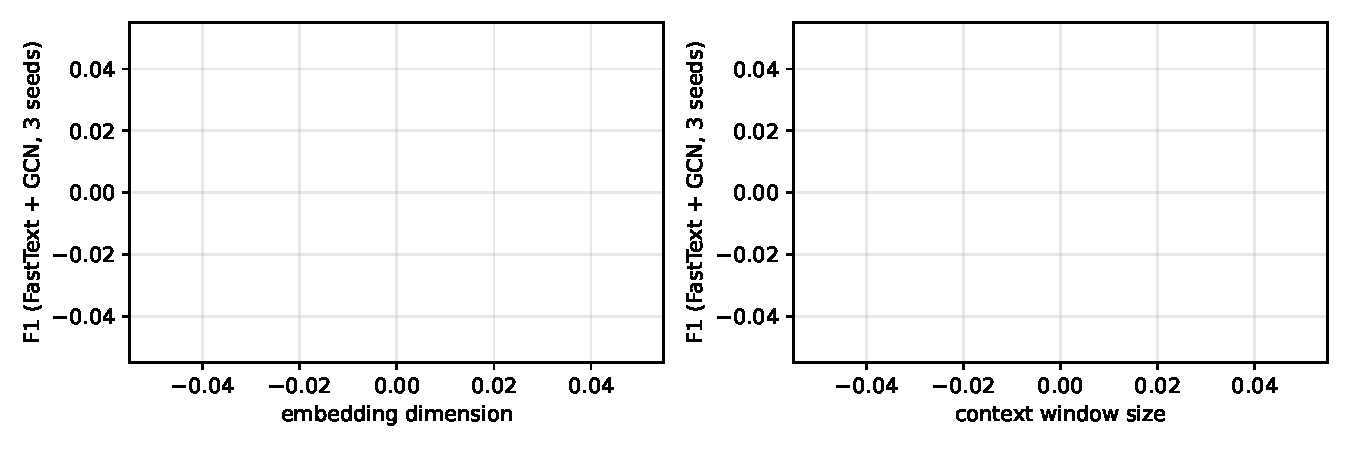
\includegraphics[width=0.72\linewidth]{figures/sweeps.pdf}
\caption{Embedding dimension (left) and FastText context window (right) vs.\ F1, FastText + GCN on \pr, 3 seeds
(cf.\ paper Fig.~6 and 7). Error bars: 95\% CI.}\label{fig:sweeps}
\end{figure*}
\begin{figure*}[!t]\centering
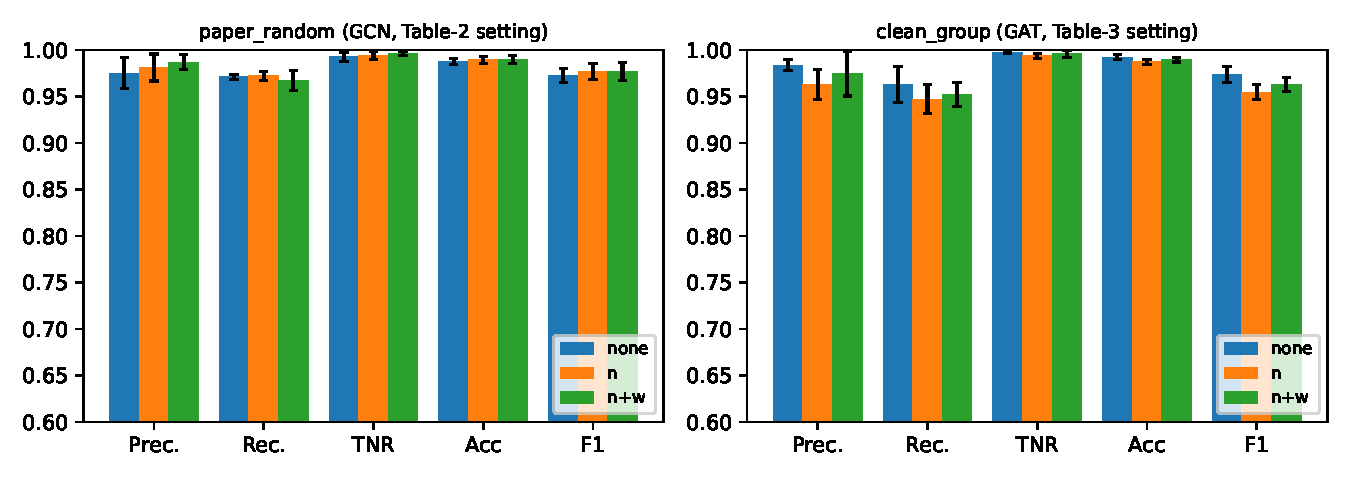
\includegraphics[width=0.78\linewidth]{figures/ablation.pdf}
\caption{Ablation of normalisation and risk weights on both protocols (cf.\ paper Fig.~8).}\label{fig:ablation}
\end{figure*}
\begin{table*}[!t]\centering\footnotesize
\caption{Paired significance tests (5 seeds, same test files). ``Significant'': paired-$t$ $p<0.05$.}\label{tab:signif}
\begin{tabular}{@{}llrrrr@{}}
\toprule
Protocol & Comparison (A vs B) & $\Delta$F1 (A$-$B) & paired-$t$ $p$ & McNemar $p<.05$ & Significant \\ \midrule
paper\_random & GAT vs GCN (Table 4) & -0.0009$\pm$0.0087 & 0.790 & 0/5 & no \\
paper\_random & GAT vs GIN (Table 4) & -0.0034$\pm$0.0123 & 0.479 & 1/5 & no \\
paper\_random & FastText vs D2V-w (Table 2) & +0.0419$\pm$0.0226 & 0.007 & 5/5 & yes \\
paper\_random & n+w vs none (GCN, Fig. 8) & +0.0040$\pm$0.0052 & 0.100 & 1/5 & no \\
clean\_group & n+w vs none (GAT, Fig. 8) & -0.0104$\pm$0.0116 & 0.068 & 1/5 & no \\
paper\_random & GAT vs TF-IDF + LR & -0.0174$\pm$0.0126 & 0.019 & 3/5 & yes \\
clean\_group & GAT vs TF-IDF + LR & -0.0291$\pm$0.0100 & 0.001 & 4/5 & yes \\
cross\_source & GAT vs TF-IDF + LR & -0.2994$\pm$0.0390 & 0.000 & 5/5 & yes \\
\bottomrule
\end{tabular}

\end{table*}

\subsection{Leakage, baselines and generalisation (RQ3, RQ4)}\label{sec:beyond}
\paragraph{Leakage and baselines (\Cref{tab:protocols})}
Removing near-duplicate leakage (\cg) lowers GNN F1 by about two points (GAT 0.980 $\to$ 0.963). A bag of lexical tokens
with logistic regression beats every GNN on every protocol (F1 0.997 / 0.992; paired $p \le 0.019$), at seconds of CPU
time and without an ICFG. Twelve graph statistics without any code semantics reach F1 0.917 on \pr: most of the
separation is available from the \emph{shape} of the ICFG. Rules from GlareShell's own risk lists are weak (F1
0.36--0.64): many benign framework files call the same functions.

\begin{table}[!t]\centering\scriptsize
\caption{GNNs and baselines (5 seeds). F1 on the paper's random split (\pr) and the clean split (\cg); FPR on 9,091 files of four unseen benign
projects and recall on 18 unseen webshells (\xs).}\label{tab:protocols}
\setlength{\tabcolsep}{3pt}
\begin{fittable}\begin{tabular}{@{}lrrrr@{}}\toprule
Model & F1 random & F1 clean & FPR unseen & Recall unseen \\ \midrule
GlareShell GCN & 0.981$\pm$.008 & 0.959$\pm$.011 & 1.84\% & 0.54$\pm$.06 \\
GlareShell GAT & 0.980$\pm$.012 & 0.963$\pm$.008 & 1.69\% & 0.64$\pm$.13 \\
TF-IDF + LR & \textbf{0.997}$\pm$.002 & \textbf{0.992}$\pm$.005 & \textbf{0.35\%} & 0.77$\pm$.03 \\
TF-IDF + XGBoost & \textbf{0.998}$\pm$.002 & 0.990$\pm$.008 & 1.34\% & \textbf{0.92}$\pm$.04 \\
Graph stats + XGB & 0.917$\pm$.008 & 0.825$\pm$.043 & 2.88\% & 0.42$\pm$.08 \\
Rule: any risky call & 0.637$\pm$.010 & 0.551$\pm$.077 & 9.98\% & 0.22 \\ \bottomrule
\end{tabular}\end{fittable}
\end{table}

\paragraph{Unseen benign projects and alarm budgets}
On \xs{} the GNN false-positive rate quadruples, from 0.4\% to 1.7\% (Joomla worst at 3\%), while TF-IDF + LR stays at
0.35\%. The threshold-free view is worse (\Cref{fig:roc}): with a 0.1\% alarm budget, the realistic budget of a
file-upload monitor, GAT recovers only \textbf{6\%} of the unseen webshells (average precision 0.11), TF-IDF + LR
\textbf{64\%} (AP 0.61). The GNN's false positives on unseen projects are \emph{confident}: they rank above most
webshells, so no threshold separates them.

\begin{figure}[!t]\centering
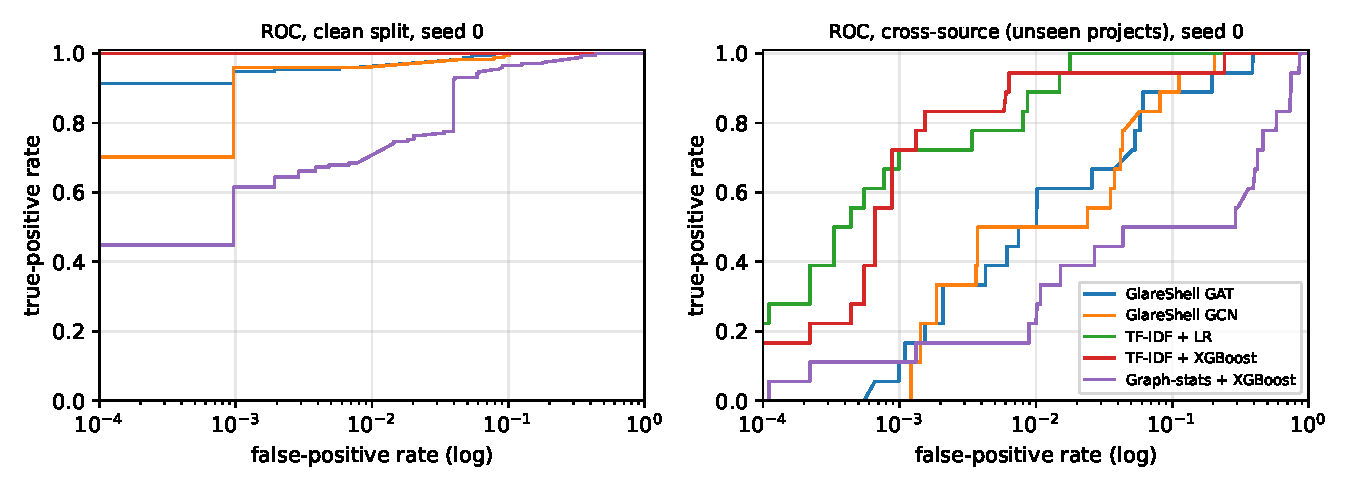
\includegraphics[width=\linewidth]{figures/roc.pdf}
\caption{ROC curves (log FPR axis), seed 0. Left: \cg; right: \xs{} (unseen benign projects, 18 unseen webshells).}\label{fig:roc}
\end{figure}

\paragraph{Unseen webshells}
Recall on the 18 novel webshells drops from 0.97 to 0.64 (GAT) and 0.54 (GCN). Holding out whole collections
(\texttt{loo}) is milder -- GNN recall 0.92--0.95 on 77--222 unseen webshells -- but TF-IDF again does better
(0.97--1.00) and even graph statistics recover 69--87\%: public collections copy from each other, so a held-out
collection is not a held-out family.

\paragraph{Small standalone benign scripts}
All benign training files come from large frameworks. We wrote 12 ordinary standalone scripts of the kind found on small
company servers (contact form, image upload with MIME check, PDO login, CSV export, JSON API, admin ping tool with
\texttt{escapeshellarg}, a three-line greeting, \dots). The final demo model (FastText + GAT, F1 0.974 and FPR 0.1\% on
its own test set) flags \textbf{10 of the 12} as webshells, most with $p > 0.98$; TF-IDF + LR flags 6 (\Cref{tab:probe}). Both detectors
have learned the population difference -- small, procedural, reads \texttt{\$\_GET/\$\_POST} -- rather than malicious
behaviour.

\begin{table*}[!t]\centering\footnotesize
\caption{Webshell probability for 12 hand-written benign standalone scripts (\texttt{tests/probe\_benign/});
models trained on \cg, seed 0. Bold: flagged ($p \geq 0.5$).}\label{tab:probe}
\begin{tabular}{@{}lrrl@{}}\toprule
Script & GAT & TF-IDF+LR & What it does \\ \midrule
hello.php & \textbf{1.000} & \textbf{0.924} & echo greeting with \texttt{htmlspecialchars} \\
contact\_form.php & \textbf{0.998} & \textbf{0.760} & validated form + \texttt{mail()} \\
download.php & \textbf{0.999} & 0.373 & whitelisted file download \\
export\_csv.php & \textbf{0.996} & \textbf{0.569} & PDO query $\to$ CSV \\
guestbook.php & \textbf{0.998} & \textbf{0.916} & append-only text file \\
image\_upload.php & \textbf{0.982} & 0.252 & MIME/size-checked upload \\
login.php & \textbf{0.930} & \textbf{0.651} & PDO + \texttt{password\_verify} \\
ping\_tool.php & \textbf{0.992} & \textbf{0.628} & \texttt{shell\_exec} with validated IP + \texttt{escapeshellarg} \\
router.php & \textbf{0.994} & 0.146 & static route table + \texttt{include} \\
template\_render.php & \textbf{0.999} & 0.201 & \texttt{extract} + \texttt{include} template \\
cleanup\_cron.php & 0.376 & 0.490 & delete old cache files \\
json\_api.php & 0.204 & 0.377 & JSON to-do list API \\ \midrule
Flagged & \textbf{10/12} & \textbf{6/12} & \\ \bottomrule
\end{tabular}
\end{table*}

\paragraph{Error analysis}
Missed webshells are mostly files the pipeline cannot see into: on \pr{} 75\% have an empty ICFG (PHP~4-era or
malformed files, encoded droppers whose payload is a string) and 86\% contain no call from the risk lists. About half
of the \xs{} misses we inspected are \emph{label noise}: helper files shipped inside a webshell kit
(\texttt{phpinfo.php}, a database class). False positives on unseen projects (769 over 5 seeds) are 62\% Joomla, and
47\% carry no risk tag at all: layout templates mixing HTML and short PHP blocks, and small event or exception class
stubs. False positives are driven by \emph{distance from the benign training projects}, not by risky code.

\subsection{Improvement: training on small benign applications}\label{sec:hard}
The analysis suggests a fix: show the model benign code that resembles the deployment. We added five small procedural
PHP applications to training (YOURLS, FluxBB, DokuWiki, Cacti, Adminer; 2,511 files) and kept four others for testing
only (OPNsense core, osTicket, MyBB, Tiny File Manager; 2,709 files), removing any file that also occurs in the main
corpus. Base and augmented models are evaluated on the \emph{same} 13,041 files (\cg{} and \xs{} tests, held-out apps,
probes). Pooled over all benign test files, the GAT false-positive rate falls from 2.5\% to 0.9\% (paired $p=0.006$)
with no significant change in recall ($p=0.25$); TF-IDF + LR falls from 1.7\% to 0.5\% but loses 2.5 recall points
(\Cref{tab:hard}). The gain carries over to the large unseen projects (1.45\% $\to$ 0.63\%). It is not a cure: GAT
still flags 8 of the 12 probe scripts, and Tiny File Manager, a legitimate single-file file manager, stays flagged.

\begin{table}[!t]\centering\scriptsize
\caption{Base (\cg{} training) vs.\ aug (+5 small benign apps); same 13,041 test files, mean over 5 seeds.}\label{tab:hard}
\setlength{\tabcolsep}{3pt}
\begin{tabular}{@{}lrrrr@{}}\toprule
 & \multicolumn{2}{c}{GAT} & \multicolumn{2}{c}{TF-IDF + LR} \\
Test group & base & aug & base & aug \\ \midrule
All benign files: FPR & 2.52\% & \textbf{0.92\%} & 1.71\% & \textbf{0.55\%} \\
All webshells: recall & 0.926 & 0.908 & 0.971 & 0.946 \\
Unseen large projects: FPR & 1.45\% & 0.63\% & 0.34\% & 0.15\% \\
osTicket: FPR & 7.35\% & 1.32\% & 12.26\% & 3.67\% \\
OPNsense core: FPR & 5.67\% & 2.70\% & 0.24\% & 0.14\% \\
MyBB: FPR & 3.81\% & 1.09\% & 1.86\% & 0.19\% \\
12 probe scripts flagged & 11.2 & 8.4 & 6.2 & 3.0 \\
Tiny File Manager $p$ & 0.95 & 0.63 & 0.71 & 0.53 \\ \bottomrule
\end{tabular}
\end{table}

\section{Discussion}\label{sec:discussion}
\Cref{tab:verdict} summarises the verdicts.
\begin{table*}[!t]\centering\footnotesize
\caption{Verdict per claim of the paper and per addition of this work. \repro{Green}: reproduced;
\notrepro{red}: not reproduced; \improved{blue}: improved or extended.}\label{tab:verdict}
\begin{tabularx}{\linewidth}{@{}p{0.31\linewidth}Xl@{}}\toprule
Claim / item & Our evidence & Verdict \\ \midrule
ICFG + embedding + GNN reaches F1 $\approx$ 0.95--0.99 & F1 0.980--0.983 on the paper's protocol, 5 seeds & \repro{Reproduced} \\
FastText is the best embedding & 0.977, best of six, $p=0.007$ & \repro{Reproduced} \\
GAT is the best GNN & GCN 0.981, GIN 0.983, GAT 0.980; $p=0.79$ / $0.48$ & \notrepro{Not reproduced} \\
Dimension / window shape (Fig.~6--7) & flat; window 5 nominal maximum only & \notrepro{Not reproduced} \\
Normalisation + risk weights help (Fig.~8) & $p=0.10$ (\pr), reversed on \cg{} ($p=0.07$) & \notrepro{Not reproduced} \\
GNN beats text approaches & TF-IDF + LR better on every protocol, significant & \notrepro{Not reproduced} \\
Cheap enough for online monitoring & 11\,ms extraction + ms scoring per file & \repro{Reproduced} \\ \midrule
Extractor for PHP~8 code & four LChecker fixes, documented & \improved{Improved} \\
Corpus, leakage control, new protocols & GlareShell-R; 77\% leakage; \cg, \xs, \texttt{loo} & \improved{Extended} \\
Deployment view & FPR $\times$4 on unseen projects; 6\% recall at 0.1\% FPR; 10/12 probes flagged & \improved{Extended} \\
Training on small benign applications & FPR 2.5\% $\to$ 0.9\% ($p=0.006$), recall unchanged & \improved{Improved} \\ \bottomrule
\end{tabularx}
\end{table*}

\paragraph{Threats to validity}
\emph{Internal}: the ICFG construction, risk lists and statement format are our reading of an unreleased implementation;
hyper-parameters the paper leaves open were fixed before looking at test results. \emph{Construct}: labels are
source-level -- ``webshell'' means ``from a public collection'' -- and the two populations also differ in age, size and
parseability, which a classifier can exploit; collections contain non-malicious helpers. \emph{External}: five benign
training projects (ten with the improvement) and only 18 truly novel webshells; no adaptive attacker.
\emph{Conclusion}: five seeds give limited power, so a non-significant difference means ``not shown'', not ``equal'';
only the alarm-budget operating points use test-set thresholds, which is optimistic for all models alike.

\paragraph{Safety, ethics and reproducibility}
Samples are only parsed, never executed or served; \texttt{samples/} and derived code fragments are git-ignored, the
Docker image runs with \texttt{--network none} and read-only samples, and graders receive a password-protected archive
(\texttt{infected}) with checksums. The repository contains pinned fetch scripts, the hash manifest, all splits, every
run's configuration and per-file predictions, a Dockerfile and \texttt{reproduce.sh}; \texttt{analyze.py} regenerates
every table and figure. The 125 GNN runs took about 5.3 GPU-hours on a laptop GPU.

\section{Conclusion}\label{sec:conclusion}
GlareShell's headline F1 of about 0.98 is reproducible without the authors' code or data; its finer conclusions are not,
once seeds and paired tests are used. More importantly, the benchmark mostly measures the difference between five large
frameworks and public webshell collections: 77\% of test webshells leak via near-duplicates, a lexical baseline beats
the GNNs, and the models flag most small legitimate scripts and lose almost all recall at a realistic alarm budget on
unseen projects. Training on benign code that resembles the deployment cuts false positives by a factor of almost
three. A practical detector needs such benign data at scale, cluster- and source-disjoint evaluation by default,
relabelled kit helpers, and FPR on unseen projects reported next to F1.
